\section{Strategie}

Testowanie na podstawie właściwości nie jest proste w zastosowaniu, przynajmniej przy pierwszej próbie.
Istnieją jednak pewne schematy wskazujące drogę, jak stworzyć takie testy.
\subsection{Różne ścieżki, ten sam wynik}

Jedną z podstawowych strategii skorzystanie z komutatywności niektórych operacji. Można to zrobić poprzez wykonanie operacji w różnej kolejności, jak zaprezentowano w \refrys{fig:commutative_strategy}.
\begin{figure}[h]
    \centering
    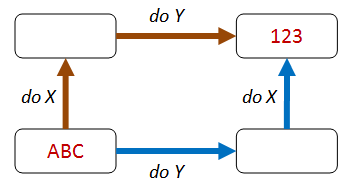
\includegraphics[width=0.5\textwidth]{images/property_commutative.png}
    \caption{Strategia - komutatywność}
    \label{fig:commutative_strategy}
\end{figure}

Przykładem takiej strategii może być komutatywność dodawania z \reflist{kod:add_all_properties}, gdzie wykorzystano \texttt{add x y}, jak i odwrotność tej operacji \texttt{add y x}. 
Innym przykładem jest test metody \texttt{sort} danej listy. 
Wykonanie sortowania, a następnie dodanie do każdego elementu listy \texttt{1} powinno dać taki sam efekt jak dodanie \texttt{1} do każdego z elementów listy, a następnie jej posortowanie \refrys{fig:commutative_strategy_list_sort} \reflist{kod:list_sort_add1}.

\begin{figure}
    \centering
    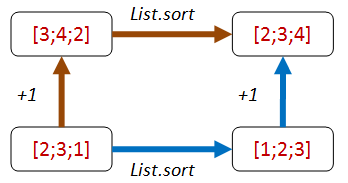
\includegraphics[width=0.5\textwidth]{images/property_list_sort1.png}
    \caption{Strategia - komutatywność - sortowanie listy}
    \label{fig:commutative_strategy_list_sort}
\end{figure}
\lstset{language=FSharp, basicstyle=\scriptsize}
\begin{lstlisting}[frame=single,caption={Test sortowania listy z wykorzystaniem strategii komutatywnej},label=kod:list_sort_add1]
    let addThenSort_eq_sortThenAdd sortFn aList =
        let add1 x = x + 1

        let result1 = aList |> sortFn |> List.map add1
        let result2 = aList |> List.map add1 |> sortFn
        result1 = result2
\end{lstlisting}

\subsection{Tam i z powrotem}
    